\documentclass[twocolumn,usenames,dvipsnames]{aastex63}

\usepackage{graphicx}
\usepackage{verbatim}
\usepackage{color}
\usepackage{natbib}
\usepackage{shortbold}
\usepackage{booktabs}
\usepackage{tabularx}
\usepackage{hyperref}
\usepackage{amsmath}
\usepackage{array}
\usepackage{multirow}
\usepackage{makecell}
\usepackage[normalem]{ulem}
\usepackage{xspace}
\usepackage{xcolor}

\newcommand{\cheung}[1]{\textcolor{red}{{#1}}}
\newcommand{\bose}[1]{\textcolor{blue}{{#1}}}
\newcommand{\miho}[1]{\textcolor{green}{#1}}

\usepackage{colortbl,dcolumn}

\def\zz#1{%
\ifdim#1pt>89pt\cellcolor{green}\else
\ifdim#1pt>79pt\cellcolor{yellow}\else
\cellcolor{OrangeRed}\fi\fi
#1}


\begin{document}

\title{Multi-Channel Auto-Calibration for the Atmospheric Imaging Assembly with Deep Learning}

\author{Luiz F. G. dos Santos}
\affil{The Catholic University of America, 620 Michigan Avenue NE, Washington, DC 20064, USA}
\affil{Heliophysics Science Division, NASA, Goddard Space Flight Center, Greenbelt, MD 20771, USA}
\author{Souvik Bose}
\affil{Rosseland Center for Solar Physics, University of Oslo,P.O. Box 1029 Blindern, NO-0315 Oslo, Norway}
\affil{Institute of Theoretical Astrophysics, University of Oslo,P.O. Box 1029 Blindern, NO-0315 Oslo, Norway}
\author{Brad Neuberg}
\affil{Frontier Development Lab, Mountain View, CA 94043, USA}
\affil{SETI Institute, Mountain View, CA 94043, USA}
\author{Valentina Salvatelli}
\affil{Frontier Development Lab, Mountain View, CA 94043, USA}
\affil{SETI Institute, Mountain View, CA 94043, USA}
\author{Mark C. M. Cheung}
\affil{Lockheed Martin Solar \& Astrophysics Laboratory (LMSAL), Palo Alto, CA 94304, USA}
\author{Miho Janvier}
\affil{Universit\'e Paris-Saclay, CNRS, Institut d'astrophysique spatiale, Orsay, France}
\author{Meng Jin}
\affil{SETI Institute, Mountain View, CA 94043, USA}
\affil{Lockheed Martin Solar \& Astrophysics Laboratory (LMSAL), Palo Alto, CA 94304, USA}
\author{Yarin Gal}
\affil{OATML, Department of Computer Science, University of Oxford, Oxford OX1 3QD, UK}
\author{At{\i}l{\i}m G\"{u}ne\c{s} Bayd{\rlap{\.}\i}n}
\affil{Department of Engineering Science, University of Oxford, Oxford, Oxford OX1 3PJ, UK}



\keywords{Sun: Solar extreme ultraviolet emission; Solar active regions;  -- methods: GPU computing; Convolutional neural networks; }

\begin{abstract}


Solar activity plays a quintessential role in influencing the interplanetary medium and space-weather around the Earth. Remote sensing instruments on-board heliophysics space missions provide a pool of information about the Sun’s activity, via the measurement of its magnetic field and the emission of light from the multi-layered, multi-thermal and dynamic solar atmosphere. Extreme UV (EUV) wavelength observations from space help in understanding the subtleties of the outer layers of the Sun, namely the chromosphere and the corona. Unfortunately, such instruments, like the Atmospheric Imaging Assembly (AIA) onboard NASA’s Solar Dynamics Observatory (SDO), suffer from time-dependent degradation that reduces their sensitivity. Current state-of-the-art calibration techniques rely on periodic sounding rockets which can be infrequent and rather unfeasible for deep-space missions. As a part of Frontier Development Lab, we devised a convolutional neural network (CNN) based approach to calibrate, as an alternate to the sounding rocket missions. We use SDO-AIA data for our analysis that aims to perform the auto-calibration by exploiting spatial patterns on the solar surface across multi-wavelength observations. Our results show that CNN based models could comprehensively reproduce the outcomes of the sounding rocket experiments within a reasonable degree of accuracy, indicating that it performs equally well when compared with the current techniques. Furthermore, comparison with a standard “astronomer’s technique” (baseline model) reveal that the CNN approach outperforms it quite significantly. This approach establishes the framework for a novel technique to calibrate EUV instruments and advance our understanding of the cross-channel relation between different EUV channels. 
\end{abstract}

\section{Introduction}
\label{Section:intro}
Solar activity plays a significant role in influencing the interplanetary medium and space weather around Earth and all the other planets of the solar system \citep{Schwenn2006}. Complex mechanisms govern such dynamic phenomena, which are crucial and challenging to understand. Remote-sensing instruments onboard heliophysics missions can provide a wealth of information on the Sun’s activity, primarily via capturing the emission of light from the multi-layered solar atmosphere and the measurement of magnetic fields.

\begin{figure*}[ht!]
    \includegraphics[width=7.1in]{Channels_Horizontal.pdf}
    \caption{Set of images to exemplify how degradation affects the AIA images. The two sets are composed of seven images from different EUV channels. From left to right: AIA 94~\AA, AIA 131~\AA, AIA 304~\AA, AIA 335~\AA, AIA 171~\AA, AIA 193~\AA, and AIA 211~\AA. The top row corresponds to images from May $13^{th}$, 2010 and the bottom row shows images from August $31^{st}$, 2019, with no degradation correction. The 304~\AA~channel images are in log-scale due the severe degradation.}
    \label{fig:autocalibrate_model_problem}
\end{figure*}

NASA currently manages the Heliophysics System Observatory (HSO), which consists of a group of satellites constantly monitoring the Sun, its extended atmosphere, space environments around the Earth and other planets of the solar system \citep{HSO}. One of the flagship missions of HSO is NASA's Solar Dynamics Observatory (SDO) \citep{SDO_primary}. Launched in 2010, SDO has been instrumental in monitoring the Sun's activity and providing valuable scientific data every day with a high temporal and spatial resolution. It has three instruments onboard: the Atmospheric Imaging Assembly (AIA) \citep{AIA}, which records high spatial and temporal resolution ultraviolet (UV) and extreme UV (EUV) images of the Sun; the Helioseismic \& Magnetic Imager (HMI) \citep{HMI}, providing context high-resolution magnetograms; and the EUV Variability Experiment (EVE) \citep{EVE}, which measures the solar EUV spectral irradiance.

Over the past decade, SDO has played a central role in advancing our understanding of the fundamental plasma processes governing the Sun and space weather. This success can mainly be attributed to the open-data policy and a consistent high data-rate of approximately two terabytes of scientific data per day. The large volume of data accumulated over the past decade (over 12 petabytes) provides a fertile ground to develop and apply new data processing methods that can further expand the capabilities of SDO.

In Figure \ref{fig:autocalibrate_model_problem} there are sample images from the seven EUV channels in AIA. On the top row we observe the first images captured by AIA, in May $13^{th}$ of 2010, and in the bottom row the images captured more recently in August $31^{st}$, 2019. It is possible to observe the more recent images are dimmer than the first ones obtained by AIA, more intensly in 304~\AA~ channel, even though plotted in the same intensity range. This effect is due to the temporal degradation EUV instruments suffer. These instruments in space are known to suffer degradation, which diminishes overall instrument sensitivity with time~\citep[e.g.,][]{BenMoussa_etal_2013}. The possible causes include the out-gassing of organic materials in the telescope structure \citep{Jiao_2019}, which may deposit on optical elements or the decrease in detector sensitivity due to exposure to EUV radiation. In general, first-principles models predicting the sensitivity degradation as functions of time and wavelength are not sufficiently well-constrained for maintaining the scientific calibration of the instruments. Instrument teams have, therefore, traditionally relied on empirical techniques, such as relying on sources with known fluxes. However, there are no standard candles on the Sun at these wavelengths. Quiet Sun EUV brightness is variable depending on the configuration of the small-scale fields. Furthermore, the quiet Sun may be too dim in some EUV channels (e.g., the 94~\AA\ channel in AIA). Active regions (ARs) are brighter than the quiet Sun, but EUV fluxes from ARs can vary by orders of magnitude depending on whether the AR is emerging, flaring or decaying, and on the AR's magnetic complexity.

 Current methods to compensate for this degradation include sounding rocket experiments \citep{EVE_rocket} that use a near-replica of the instrument on-board SDO to gather a calibrated observation spanning the short interval of the suborbital flight (a few minutes). A comparison of the sounding rocket observation with the orbital satellite’s observation provides an updated calibration, revealing long-term trends in the sensitivities of EVE and AIA. Sounding rockets are undoubtedly crucial. However, the sparse temporal coverage and the complexities of intercalibration are also sources of uncertainty inter-instrument calibration. Moreover, it may not be practical for missions in deep space \citep[e.g., STEREO,][]{Kaiser_2008}.
 
 The application of machine learning (ML) \citep{bishop2006pattern} has gained momentum in the space weather community and it is driving an intense development of automated technologies to improve data processing, and assimilation in solar physics. Recent studies including, predicting solar flares from HMI vector magnetic fields \citep{Bobra_2015}, creating high-fidelity virtual observations of the solar corona \citep[\citealt{salvatelli2019} \&][]{Cheung2019}, forecasting far side magnetograms from STEREO EUV images \citep{Kim_NatAs_2019}, super-resolution of magnetograms \citep{jungbluth-2019-super}, mapping EUV images from AIA to spectral irradiance measurements \citep{Szenicereaaw6548} and the early stages of this project \citep{neuberg2019} have demonstrated the immense potential of ML applications in solar and heliophysics. In this paper, we focus on automating the correction of the sensitivity degradation of different AIA wavebands by using a deep neural network \citep{goodfellow2016deep} that exploits spatial patterns and cross-spectral correlations in multi-wavelength observations. The approach developed in this work removes a significant impediment to developing future HSO missions that can deliver solar observations from different vantage points beyond Earth-orbit.
 
This paper is structured as follows: In Section \ref{Section:data}, we present and describe our data set used, in section \ref{section:methodology} we formulate the problem (\S~\ref{section:formulation}), present the CNN model(\S~\ref{section:convolutional}), probe the multi-channel relationship (\S~\ref{section:inter_channel}) and explain the training process and evaluation (\S~\ref{Section:Analysis}). In section \ref{section:baseline} we present the baseline, followed by section \ref{Section:Results} where we present the results and discussions. The conclusion and summary is in section \ref{section:summary}.
 
\section{Data description}
\label{Section:data}

We use the pre-processed SDO/AIA dataset from \citet{SDOML} (hereafter referred to as SDOML). This dataset is ML-ready to be used for any kind of application related to the AIA and HMI data and consists of a subset of the original SDO data dating from 2010 to 2018. It comprises of the $7$~EUV channels, $2$~UV channels from AIA and vector magnetograms from HMI. The data from both the instruments have been spatially aligned, and have identical temporal sampling with a spatial sampling of $\thicksim$ $4\farcs8$ per pixel. Data from the three SDO instruments are temporally aligned, with cadences chosen to be 6 minutes for AIA (instead of the original 12 seconds) and EVE, and 12 minutes for HMI. The full disk images were downsampled from 4096 $\times$ 4096 to 512 $\times$ 512 pixels to have a more manageable data set.

AIA images have been normalized by exposure time and corrected for instrumental degradation over time \citep[using V8 degradation curve from sounding rocket experiments,][]{Boerner2013}. Consequently, the resulting dataset offers images where changes in pixel brightness are directly related with the state of the Sun, rather than instrument performance.

In this study, we re-sample the SDOML dataset and scale it further down to $256\times256$ pixels from $512\times512$ pixels. This enabled to  speed-up the processing and iteration times in our development of the new ML technique, besides allowing us to conserve the necessary computational resources. We also masked the off-limb signal ($r>R_\odot$) to avoid possible contaminating due to effects of telescope vignetting. In addition, we also re-scaled the brightness intensity of each AIA channel by dividing the images by a channel-wise constant factor. These factors represent the approximate median brightness in each channel and across the full time period \citep[derived from][]{SDOML}, and this process is implemented to set the brightness close to unity that makes numerical computation in the CNN much more stable. This is helpful especially in the back-propagation of the parameter values. It is a standard practice in CNNs, see for example Chapter 6 of \citep[][]{goodfellow2016deep}. The specific values for each channel are reported in Appendix~\ref{section:appendix_average}.

\section{Methodology}
\label{section:methodology}
\subsection{Formulation of the problem}
\label{section:formulation}
The approach to the problem is explained as follows. We consider a set $\vec{C} = \{C_i, i\in [1,...,n]\}$ of multi-channel, synchronous SDO/AIA images where $C_i$ denotes the $i$-th channel image in the set. Further we create a corresponding set of dimmed images as $\mathbf{\alpha} \vec{C} = \{\alpha_i C_i, i\in [1,...,n]\}$, where each dimming factor $\alpha_i$ is independently sampled from a uniform distribution between [$0.01, 1.0$]. We choose a maximum $\alpha$ =1 since we only consider dimming of the images and not enhancements. It is also to be noted that the dimming factors $\alpha_i$ are applied uniformly per channel and are not spatially dependent. The spatial dependence portion of the degradation is assumed to be accounted for by regularly updated flat-fields applied to AIA images. The goal is to find a deep learning model $M: \vec{C} \rightarrow \mathbf{\alpha}$, i.e. a deep learning model that retrieves the set of multi-channel dimming factors from observed SDO/AIA images $\vec{C}$.

\subsection{Convolutional Neural Network Model}
\label{section:convolutional}
Deep learning is a very active sub-field of machine learning that focuses on specific models called deep neural networks (DNNs).A DNN is a composition of multiple layers of linear transformations and non-linear element-wise "activation" functions \citep{goodfellow2016deep}. One of the main qualities of deep learning is that it can learn from the data the best feature representation for a given task, without the need to manually engineer features. DNNs have produced state-of-the-art results in many complex tasks including object detection in images \citep{he2016deep}, speech recognition \citep{amodei2016deep} and synthesis \citep{oord2016wavenet}, and translation between languages \citep{wu2016google}. A DNN expresses a differentiable function $F_{\mathbf\theta}: \mathcal{X} \to \mathcal{Y}$ that can be fitted to perform complex non-linear transformations, by tuning parameters $\vec{\theta}$ using gradient-based optimization of a loss (also known as objective or error) function $L(\vec{\theta}) = \sum_i l(F_{\vec\theta}(\vec{x}_i), \vec{y}_i)$ for a given set of inputs and desired outputs $\{\vec{x}_i, \vec{y}_i\}$.

For the degradation problem summarized in Section~\ref{section:formulation}, we consider two CNNs architecture \citep{lecun1995convolutional} --one that  doesn't exploit the spatial dependence across multi-channel AIA images and a second that does. The first model considers a single channel as input in the form of $(1,256, 256)$, where \textit{S} is the resolution of the image, whereas the second model takes in multiple AIA channel images at the same time as input in the form of $(n, 256, 256)$, where \textit{n} is the number of channels as indicated in Fig.~\ref{fig:autocalibrate_CNN_arch}. 

We exploit the hypothesis that a relationship exists between the spatial morphological features and the brightness of solar structures across single or multiple channels of AIA, that can then be used to accurately estimate the dimming factors. The first model ignores any possible relationship that different AIA channels might have, exploring only relationship across structures in a single channel, whereas the second one could exploit multi-channel correlations while training.

\begin{figure}[h]
    \centering
        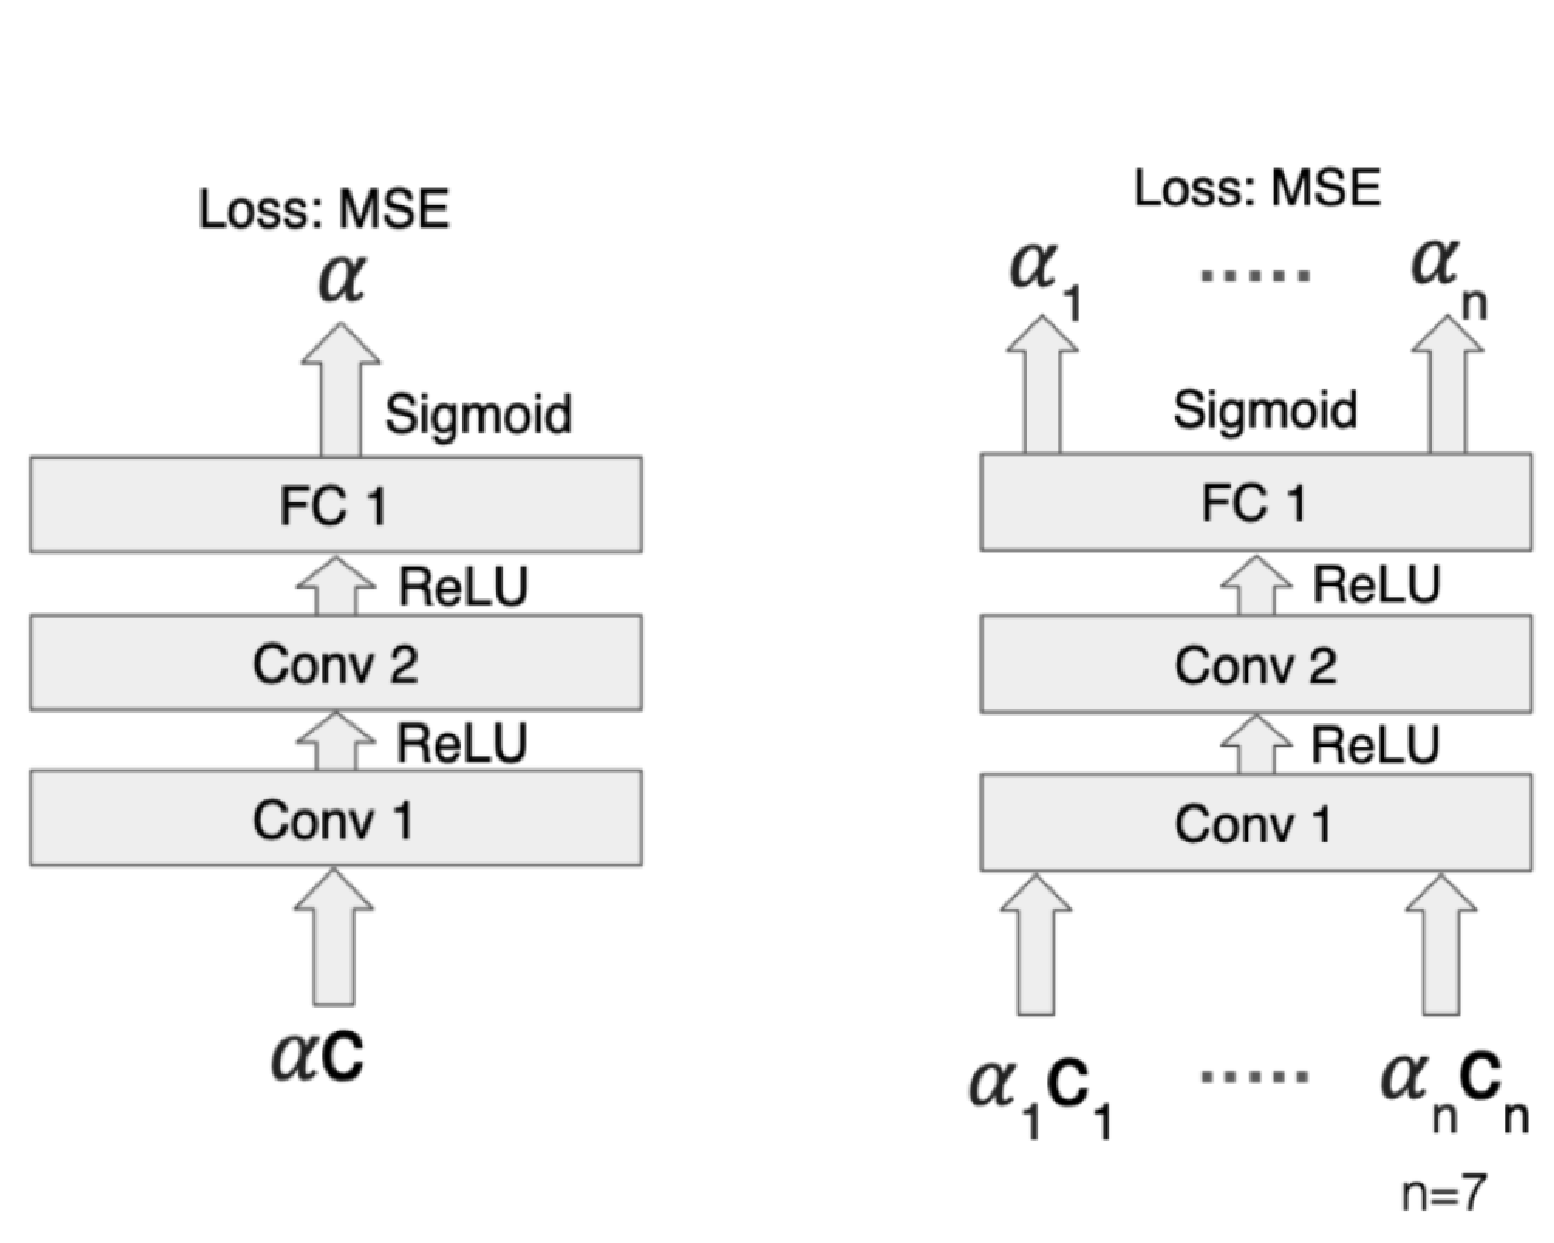
\includegraphics[height=2.7in]{archs_combined.pdf}
        \caption{The CNN architectures composed of two blocks of a convolutional layer, max pooling layer and a ReLU activation function, followed by a fully connected (FC) layer and a final sigmoid activation function.}
        \label{fig:autocalibrate_CNN_arch}
\end{figure}
	
The architecture of the CNNs (Fig. \ref{fig:autocalibrate_CNN_arch}) consists of two blocks of a convolutional layer, a max pooling layer and a ReLU(Rectified Linear Units) activation function \citep{Nair:2010:RLU:3104322.3104425}, followed by a fully connected (FC) layer, and a final sigmoid activation function. The first convolution block has 64 filters, while the second convolution block has 128. Both convolution layers use stride $ = $ 1, padding $ = $ 0, and kernel size of $3\times3$. The final configurations of the models' architectures were obtained through a grid search among different parameters and layers' configuration. 

Each CNN model takes \textit{n} (n=1 for the single channel) AIA wavelength channels as input and computes a vector of degradation factors, one for each input channel, as represented in the schematic on  Fig.~\ref{fig:autocalibrate_CNN_arch}. The second hypothesis tested here is that the multi-channel CNN can learn more effectively than a single channel CNN by simultaneously accounting for solar surface features appearing across the different channels. 

We use the open-source software library named PyTorch \citep{paszke_2017} for both training and inference purposes of the CNN.

\subsection{Probing the multi-channel relationship with a toy model}

\label{section:inter_channel}

% The reason that motivates the choice of a deep learning approach to solve this problem is that a , that can be learned through data and be used to infer the dimming factors accurately. 

In order to test the hypothesis that a physical relationship between the morphology and brightness of solar structures (e.g., active regions, coronal holes) across multiple AIA channels would help the model prediction, we generated artificial solar images, in which a 2D Gaussian profile is used (Equation \ref{E-relationship}) to mimic the Sun as an idealized bright disk with some center-to-limb variation:

\begin{equation}
\label{E-relationship}
    C_i[x,y] = A_i \exp{(-[x^2+y^2]{\sigma^{-2}})},
\end{equation}

where $A$ is the amplitude centered at (0,0), characteristic width $\sigma$, and $x$ and $y$, are the coordinates at the image. $\sigma$ is sampled from a uniform distribution between 0 and 1. These images are not meant to be a realistic representation of the Sun. However, as formulated in Eq.~\ref{E-relationship}, they include two qualities we posit to be essential for allowing our auto-calibration approach to be effective. The first is the correlation of intensities across wavelength channels (i.e., ARs tend to be bright in multiple channels). The second is the existence of a relationship between the spatial morphology of EUV structures with their brightness. This toy data set is designed so that we can independently test how the presence of (a) a relation between brightness $A_i$ and size $\sigma$, and  (b) a relation between $A_i$ for various channels; and the presence of both (a) and (b) influences performance. To evaluate this test we will use the Mean Squared Error loss (MSE loss) and expect the presence of both (a) and (b) to minimize it.

The test result of the multi-channel model with artificial solar images is shown in Table~\ref{table:toy_problem_metrics}. We can see that when $A_0 \propto \sigma$ (linear relation between size and brightness) and $A_i = A_0^i$ (i.e. dependence across channels), the CNN solution delivered minimal MSE loss (top-left cell). Eliminating the inter-channel relationship (i.e., each $A_i$ was randomly chosen) or the relation between brightness $A_i$ and size $\sigma$, the performance suffered increasing the MSE loss. Ultimately, when both $A_i$ and $\sigma_i$ were randomly sampled for all channels, the model performed equivalently to randomly guessing/regressing (bottom-right cell). These experiments confirm our hypothesis and indicate that a multi-channel input solution will outperform a single-channel input model, in presence of relationships between the morphology of solar structures and their brightness across the channels. 

\begin{table}[h]
\centering
\caption{The Mean Squared Error (MSE) for all combinations proposed in Section \ref{section:inter_channel}. The top-left cell is for the scenario when there exists a cross-channel correlation and a relation between brightness and size of the artificial Sun. The top-right cell, has is the loss with a cross-channel correlation but not the relation between brightness and size. The bottom left cell has the loss when there is no cross-channel correlation, but it has a relation between brightness and size. The bottom right cell presents the loss when the parameters are freely chosen.}
\label{table:toy_problem_metrics}
\begin{tabular}{|cc|c|l|}
\hline
 &
   &
  \multicolumn{2}{c|}{\begin{tabular}[c]{@{}c@{}}Brightness and size\\ correlation\end{tabular}} \\ \cline{3-4} 
                       &    & Yes   & No    \\ \hline
\multicolumn{1}{|c|}{\multirow{2}{*}{\begin{tabular}[c]{@{}c@{}}Cross-channel\\ correlation\end{tabular}}} &
  Yes &
  0.017 &
  0.023 \\ \cline{2-4} 
\multicolumn{1}{|c|}{} & No & 0.027 & 0.065 \\ \hline
\end{tabular}%
\end{table}

\subsection{Data Splitting, Evaluation Metric and Training}
\label{Section:Analysis}
The actual dimming factors $\alpha_i(t)$ (where $t$ is the time since the beginning of the SDO mission) trace a single trajectory in an $n$-dimensional space starting with $\alpha_i(t=0)=1$ $\forall$ $i\in[1,...,n]$ at the beginning of the mission. During training, we intentionally exclude this time-dependence from the model. This is done by (1)~using the SDOML dataset which has already been corrected for degradation effects, (2) not assuming any relation between $t$ and $\mathbf{\alpha}$ and not using $t$ as an input feature, and (3) temporally shuffling the data used for training.

The training set comprises of multi-channel images~$\mathbf{C}$ obtained during the months of January to August from 2010 to 2013 (three years) obtained every 6 hours (per day), amounting to a total of $18970$ images in $2710$ timestamps. We devised a strategy such that from one training epoch to the next, the same set of multi-channel images $\mathbf{C}$ can be dimmed by a completely independent set of $\mathbf{\alpha}$ dimming factors. This is a data augmentation procedure which allows the model to generalize and be efficient in recovering dimming factors over a wide range of solar conditions.  We used the Adam optimizer \citep{Optimizer} in our training with an initial learning rate of $0.001$ and the mean squared error (MSE) of the distance between the predicted degradation factor and the ground truth value was used as a loss (cost) function. The model was trained using 64 samples per batch and the training has been performed over $1000$ epochs.

The validation dataset, or the sample of data used to provide an unbiased evaluation of a model fit on the training dataset, holds images obtained during the months of September to October between  $2010$ and $2013$, again every 6 hours per day, totalling $9422$ images over $1346$ timestamps. The split by month between the training and validation data has a two fold objective --(1) it prevents the bias due to the variation in the solar cycle thereby allowing the model to be deployed in future deep space missions forecasting $\alpha$ for future timesteps, and (2) it ensures that the same image is never present in both the data sets (sub-sequential images will approximately be the same), leading to a more precise and a comprehensive evaluation metric.

 After training, the results of the learning algorithm are binarized using five different thresholds: the absolute value of 0.05 and relative values of 5\%, 10\%, 15\%, and 20\%. If the $|\alpha_P - \alpha_{GT} |$ is smaller than the threshold, it is considered correct $\alpha_P$; otherwise, it is incorrect. We then evaluate the binarized results by using the so-called True Positive (TP) rate, which is the ratio of correct $\alpha_P$ and total amount of $\alpha_{P}$. We chose different TP rate thresholds to gauge model success, which all them are smaller than the uncertainty of the AIA degradation \citep[aproximately 25\%, ][]{AIA_calib_paper}.

We also compare the results of the final algorithm against the degradation curves from the years $2013$ to $2020$. 

\section{Baseline Model}
\label{section:baseline}

We compare our DNN approach to a baseline motivated by the assumption that the EUV intensity outside magnetically active regions and in the quiet Sun is invariant in time 
\citep[a similar approach is also considered for the in-flight calibration of some UV instruments, e.g.][]{Schule1998}. This approach, which does not depend on  machine learning, allows us to assess our proposed solution and compare the performance of our DNN-based model. 

\begin{figure}[h]
    \centering
        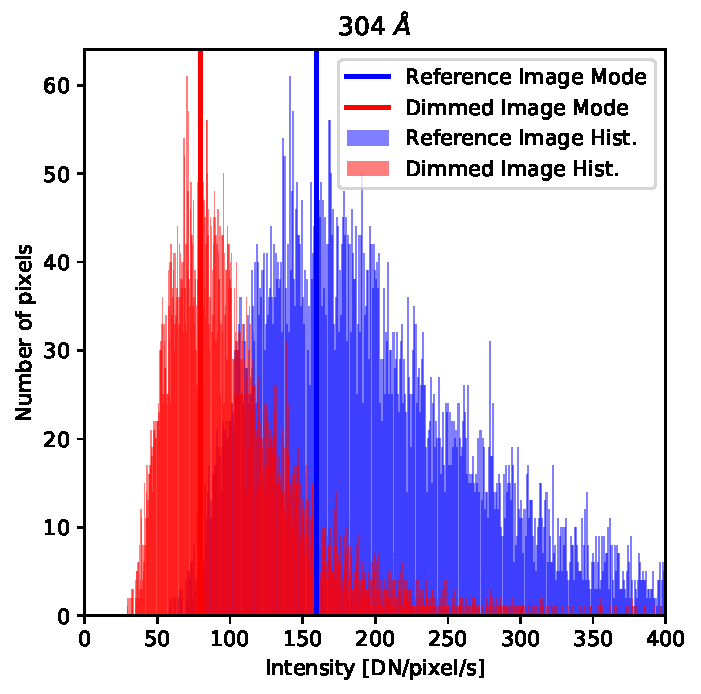
\includegraphics[height=3.3in]{hist_demo.pdf}
        \caption{Histograms (probability density functions) of the pixel values for $304~\AA$  channel. In blue the histogram for the refence image and in red the histogram for the dimmed image. The y-axis is the number of pixels, and the x-axis is the pixel intensity [$DN/px/s$]. The modes are marked with blue and red line for the reference and dimmed images respectively.}
        \label{fig:baseline_histogram}
\end{figure}

We use exactly the same data processing and splitting approach like the neural network model in Sect.~\ref{Section:Analysis}. From the processed dataset, a set of reference images per channel, $\mathbf{C_{\rm ref}}$, are selected at time $t=t_{\rm ref}$. Since the level of solar activity continuously evolves in time, we only select the regions of the Sun that correspond to low activity, as discussed in the preceding paragraph. The activity is decided based on co-spatial magnetic field maps from HMI and EUV images from AIA. To define these regions, we first pre-process the images by making a square selection with a diagonal $= 2R_\odot$ centered at $R=0$ of the solar images, so as to avoid any limb or LOS projection effects. Further, we apply an absolute global threshold value of  $5$ Mx~cm$^{-2}$ on the HMI LOS magnetic field maps corresponding to $t=t_{\rm ref}$, such that only those pixels that have B$_{\mathrm{LOS}}$ less than the threshold are extracted resulting in a binary mask where the value of $1$ corresponds to the pixels of interest and $0$ the rest. Finally, we use this mask to extract the co-spatial quiet Sun pixels from each AIA channel and compute 1D histograms of the pixel intensity values. Two such histograms are shown in Fig.~\ref{fig:baseline_histogram} for AIA $131$~\AA\ and 304~\AA\, respectively.

Upon closer investigation, we find that the 1D histograms in Fig.~\ref{fig:baseline_histogram} are non-Gaussian in nature and resemble a log-normal distribution. This is also the case for all the other AIA EUV channels. We use the mode or the most probable value of intensity to define a characteristic value that can be used as a reference denoted by $I_{i,{\rm ref}}^{\rm mp}$, where \textit{i} implies the AIA channel under consideration and \textit{mp} stands for the most probable value of intensity.
Then, we apply the exact same procedure to a different batch of images each of which were dimmed by a random dimming factor $\alpha_i$ and obtain $I^{\rm mp}_{i}$ as the most probable intensity value from its distribution. Finally, the baseline computes the ration between the two most probable intensity values and obtains the dimming factors according to the following equation:

\begin{equation}
    \alpha_i := \frac{I^{\rm mp}_{i}}{I_{i, {\rm ref}}^{\rm mp}}
\end{equation}

% Each of the images obtained is then compared to the reference image (the image at $t_{ref}<t_{i}$ for each $i$), and for each separate channel.  

% Then, the baseline model estimates the dimming factors according to the following relation: 

% \begin{equation}
%     \alpha_i := \frac{I^{\rm mp}_{i}}{I_{i, {\rm ref}}^{\rm mp}}
% \end{equation}

The efficiency of the baseline in recovering the dimming factor is then evaluated according to the TP rate metric and the results for all channels are tabulated in Table~\ref{tab:autocalibrate_final_results}. 

\section{Results and Discussions}
 \label{Section:Results}

\subsection{Comparing the performances of the baseline model with different CNN architectures}
The baseline, single-channel, and multi-channel model results are summarized in Table~\ref{tab:autocalibrate_final_results}. The different colors are for different TP rates: green is for TP rates greater than 90\%, yellow for TP rate between 80\% and 90\%, and red is for TP rate lower than 80\%. In a overview, the result shows that higher TP rates for the CNN models, particularly for the Multi-Channel model, and for higher tolerances, which is expected.

\begin{table*}[ht!]
  \centering
  \caption{Results of the baseline and CNN models applied to all the EUV AIA channels. The Table is divided in three sections: Baseline, Single Channel and Multi-Channel model. From left, the channel number, the True Positive rates for the baseline, the True Positives rates for the single channel CNN model, and the True Positive rates, for the multi-channel CNN model, each model performance is considered at different tolerance levels. At the bottom, the mean of the True Positive rate across all the channels. Color green is for TP rates greater than 90\%, yellow for TP rate between 80\% and 90\% and red is for TP rate lower than 80\%.}
  \label{tab:autocalibrate_final_results}
  \centering
  \begin{tabular}{cccccccccccccccc}
    \toprule
    \multirow{2}{*}{Channel} & \multicolumn{5}{c}{\parbox{5cm}{\centering Baseline}} & \multicolumn{5}{c}{\parbox{5cm}{\centering Single Channel Model}} &  \multicolumn{5}{c}{\parbox{5cm}{\centering Multi-Channel Model}}  \\
    \cmidrule(lr){2-6}\cmidrule(lr){7-11}\cmidrule(lr){12-16}
     & 0.05 & 5\% & 10\% & 15\% & 20\% & 0.05 & 5\% & 10\% & 15\% & 20\% & 0.05 & 5\% & 10\% & 15\% & 20\%\\
     \midrule
     94~\AA  & \zz {28}\% & \zz {08}\% & \zz {16}\% & \zz {26}\% & \zz {37}\% & \zz {70}\% & \zz {37}\% & \zz {61}\% & \zz {78}\% & \zz {87}\% & \zz {82}\% & \zz {48}\% & \zz {73}\% & \zz {85}\% & \zz {92}\% \\
     131~\AA & \zz {76}\% & \zz {49}\% & \zz {72}\% & \zz {86}\% & \zz {96}\% & \zz {94}\% & \zz {72}\% & \zz {92}\% & \zz {98}\% & \zz {99}\% & \zz {99}\% & \zz {76}\% & \zz {94}\% & \zz {97}\% & \zz {99}\% \\
     171~\AA & \zz {56}\% & \zz {27}\% & \zz {48}\% & \zz {68}\% & \zz {85}\% & \zz {93}\% & \zz {70}\% & \zz {93}\% & \zz {97}\% & \zz {99}\% & \zz {84}\% & \zz {48}\% & \zz {72}\% & \zz {86}\% & \zz {93}\% \\
     193~\AA & \zz {42}\% & \zz {13}\% & \zz {28}\% & \zz {43}\% & \zz {53}\% & \zz {73}\% & \zz {41}\% & \zz {69}\% & \zz {85}\% & \zz {93}\% & \zz {90}\% & \zz {59}\% & \zz {85}\% & \zz {94}\% & \zz {98}\% \\
     211~\AA & \zz {31}\% & \zz {11}\% & \zz {21}\% & \zz {30}\% & \zz {40}\% & \zz {63}\% & \zz {30}\% & \zz {53}\% & \zz {71}\% & \zz {84}\% & \zz {76}\% & \zz {41}\% & \zz {68}\% & \zz {82}\% & \zz {92}\% \\
     304~\AA & \zz {87}\% & \zz {66}\% & \zz {89}\% & \zz {95}\% & \zz{100}\% & \zz {90}\% & \zz {65}\% & \zz {89}\% & \zz {97}\% & \zz {99}\% & \zz {94}\% & \zz {62}\% & \zz {86}\% & \zz {93}\% & \zz {96}\% \\
     335~\AA & \zz {37}\% & \zz {14}\% & \zz {29}\% & \zz {42}\% & \zz {51}\% & \zz {62}\% & \zz {31}\% & \zz {54}\% & \zz {69}\% & \zz {80}\% & \zz {73}\% & \zz {39}\% & \zz {65}\% & \zz {82}\% & \zz {91}\% \\
     \textbf{Mean} & \textbf{\zz {51}\%} & \textbf{\zz {27}\%} & \textbf{\zz {43}\%} & \textbf{\zz {56}\%} & \textbf{\zz {66}\%} & \textbf{\zz {78}\%} & \textbf{\zz {50}\%} & \textbf{\zz {73}\%} & \textbf{\zz {85}\%} & \textbf{\zz {92}\%} & \textbf{\zz {85}\%} & \textbf{\zz {53}\%} & \textbf{\zz {77}\%} & \textbf{\zz {89}\%} & \textbf{\zz {94}\%} \\
     \bottomrule
  \end{tabular}
\end{table*}

A detailed look at Table~\ref{tab:autocalibrate_final_results} reveals that for an absolute tolerance value of $0.05$, the best results for the baseline are 87\% (304 \AA) and 76\% (131 \AA), and a mean success rate of $\sim$51\% across all channels. As we increase the relative tolerance levels, the mean TP rate increases from 27\% (for 5\% relative tolerance) to 66\% (with 20\% relative tolerance) and with a 37\% TP rate in the worst performing channel (94 \AA).

Investigating the performance of the CNN architecture with a single input channel and an absolute tolerance level of 0.05, we find that this model performed significantly better than our baseline with much higher values of the metric, for all the channels. The most significant improvement was shown by the 171~\AA\ channel with an increase from $56\%$ in the baseline model to about 93\% in this case, for an absolute tolerance of $0.05$. The average TP rate bumped from 70\% in the baseline to 78\% in the single-channel model. The worst metric for the single-channel CNN architecture was recorded by the 211~\AA\ channel, with a TP rate of just 63\%, which is still significantly better than its baseline counterpart (38\%). Furthermore, with a relative tolerance value of 15\%, we find that the mean TP rate is 85\% for the single-channel mode, which increases to more than 90\% for a 20\% tolerance level. This is a promising result considering the fact that the errors associated with the current state-of-the-art calibration techniques (sounding rockets) is $\sim25\%$.  

Finally, we report the results from the multi-channel CNN architecture in the last section of Table~\ref{tab:autocalibrate_final_results}. As expected, the performance in this case is the best of the lot with significant improvements for almost all the EUV channels. Clearly, the TP rates belonging to the red category is much lesser compared to the former models implying that the mean TP rate is the highest across all tolerance levels. The multi-channel architecture recovers the degradation (dimming) factor for all channels with a TP rate of at least 91\% for a relative tolerance level of 20\% with a mean TP rate of $\sim94\%$. It is also evident that this model outperforms the baseline and the single-channel model for all levels of relative tolerances.  For any given level of tolerance the TP rate is consistently the worst for 335~\AA\ and 211~\AA\ channels whereas the performance of the 131~\AA\ channel is the best.
% For the same tolerance, the metrics for the worst wavelengths degradation recovery were 211 \AA~ and 335 \AA~ with 82\%. Within a tolerance of 0.05, 131 \AA~ recovers the degradation factor with rate of 99\%. 

The 304 \AA~ channel we see it does consistently good through all the models with not much variation, which is different from 171 \AA~ that does well i n the baseline and has its maximum performance in the Single Channel model, through all tolerances, and a remarkable 94\% TP rate with a tolerance of 0.05.  In opposite, 171 \AA, 211 \AA~ and 335 \AA~ channels have a poor performance in the baseline and the single-channel models, and they have a significant improvement in the Multi-Channel model.

% It is not sure what caused the drop in the performance when used the multi-channel model, even though the results are not bad, and the average over all the channels increase.

\subsection{Modelling Channel Degradation over Time}
    \label{sec:degradation}
    
In this section we discuss the results obtained when both single-channel and multi-channel CNN architectures are used to recover (predict) the instrumental degradation over time, and compare them with the actual AIA channel degradation curves $V8$ and $V9$, obtained from \textit{AIApy} Python package \footnote{https://aiapy.readthedocs.io/en/latest/?badge=latest}. We use the same SDOML dataset as discussed earlier, but this time without compensating for the channel degradation. All other pre-processing steps including masking the solar limb, rescaling the intensity etc. remain unchanged.  %The data is available at \dataset[text]{url}.


\begin{figure*}[ht!]
	\centering
		\centering
        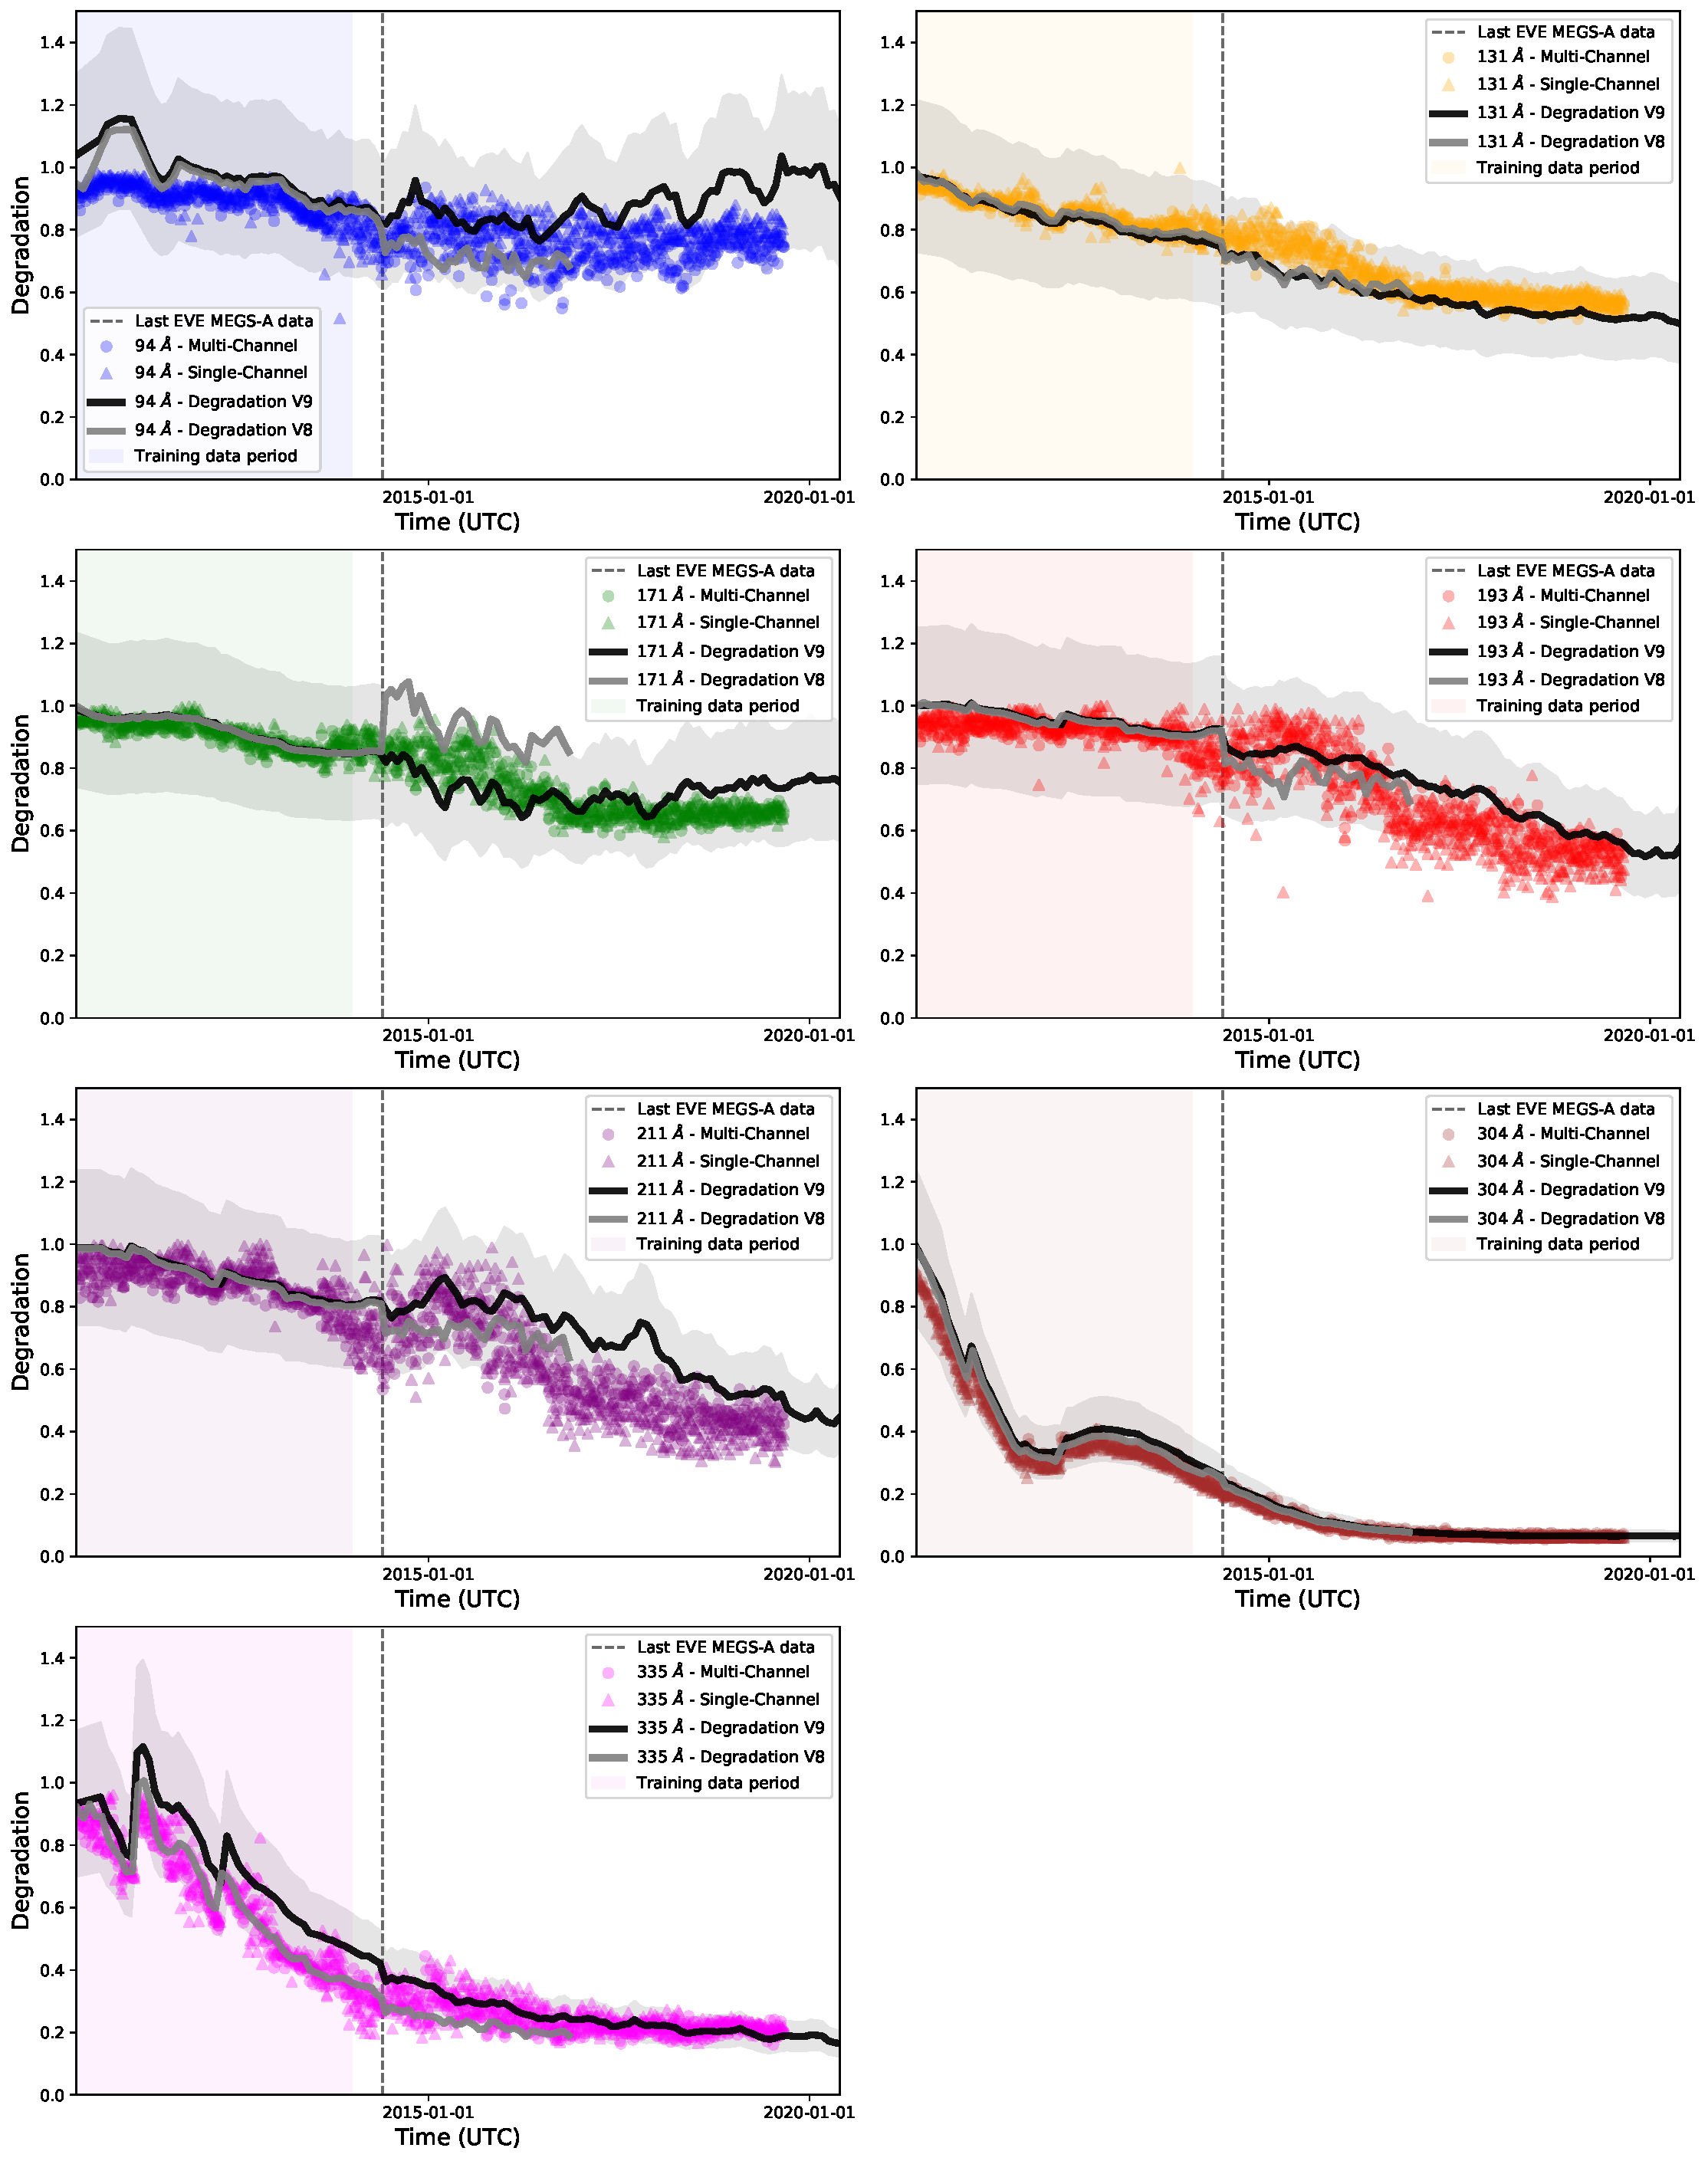
\includegraphics[width=\textwidth]{luiz_exp_36_apodize_Degradation_Alternative.pdf} 
        \caption{Channels degradation over Time. From top to bottom: Channel 94~\AA~ (blue) and 131~\AA~(yellow), 171\AA~(green) and 193~\AA~(red), 211~\AA~(purple) and 304\AA~(brown) and 335~\AA~(magenta). The black line is the degradation curve V9 and the gray line is the degradation curve V8. The gray shaded area correspond to the 25\% error of the degradation curve V9. The colorful shaded area is the training period from 2010 to 2014. The vertical dashed line is the last available observation from EVE MEGS-A data.}
        \label{fig:degradation_curve}
\end{figure*}

Figure~\ref{fig:degradation_curve} presents the results of our analysis for all the seven AIA EUV channels. In each panel, we show four quantities: the degradation curve $V9$ (solid black line), the degradation curve $V8$ (solid gray line), predicted degradation from the single-channel model (triangles) and multi-channel model (circles). The shaded gray band depicts the region covering 25\% variation (error) associated with the $V9$ degradation curve. The dashed vertical line coincides with the day (25.05.2014), when EVE MEGS-A instrument stopped working. It is important to note that MEGS-A was earlier used for the sounding rocket calibration purposes, the loss of which caused both the $V8$ and $V9$ degradation curves to become noisier. Recently, \citet{Szenicereaaw6548} addressed this aspect and used deep learning to facilitate a virtual replacement for MEGS-A.

Both the CNN models predict the degradation curves for each channel quite accurately over time as can be seen in the different panels in Fig.~\ref{fig:degradation_curve}, with the exception of 94~\AA\ and 211~\AA\ channel. However, the deviations of the predicted values fall well within the 25\% variation due to the calibration curve $V9$. 

The increased deviation in predictions for the 94~\AA\ and 211~\AA\ channels are likely due to the fact we trained both the single and multi-channel models with the SDOML dataset that was produced and corrected using the $V8$ degradation curves. The latest degradation curve ($V9$) were updated recently on July 2020 and the change from $V8$ to $V9$ might have caused an impact while training.

Comparing both single and multi-channel models, we can see that they overlap almost entirely in the temporal domain, with the single channel model predictions have a more significant variation in channel 211~\AA, 193~\AA~ and 171~\AA. For a more systematic evaluation, we calculated some good fitting metrics of both models in Table \ref{tab:quantities_degradation}.

Table \ref{tab:quantities_degradation} contains three different metrics for evaluating the good fitting of each CNN model on the V9 degradation curve. The first is the Two-Sample Kolmogorov-Smirnov Test (KS), which tests whether two samples come from the same distribution \citep{doi:10.1080/01621459.1951.10500769}. The second is the Pearson Correlation Coefficient (Pearson) that measures the linear correlation between two variables. The last metric is the Fast Dynamic Time Warping \citep[DTW, ][]{fastDTW}, which measures the similarity between two temporal sequences. This last one is important since statistical methods can be too sensitive when comparing two time series. DTW has distance between the series as an output, and for reference the DTW between the V8 and V9 degradation curves are: 94~\AA: 72.17, 131~\AA: 13.03, 171~\AA: 9.82, 193~\AA: 30.05, 211~\AA: 16.86, 304~\AA: 7.02 and 335~\AA: 5.69.

\begin{table}[h]
  \centering
  \caption{Good fitting metrics for single-channel and multi-channel models comparing to the V9 degradation curves. The first metric is the Two-Sample Kolmogorov-Smirnov Test(KS), the second one is Pearson Correlation Coefficient (Pearson), and the last one is the Fast Dynamic Time Warping which measures the similarity between two temporal sequences.}
  \label{tab:quantities_degradation}
  \centering
  \begin{tabular}{ccccccc}
    \toprule
    \multirow{2}{*}{Channel} & \multicolumn{3}{c}{{\centering Single Channel}} &  \multicolumn{3}{c}{{\centering Multi-Channel}}  \\
    \cmidrule(lr){2-4}\cmidrule(lr){5-7}
     & KS & Pearson & DTW &  KS & Pearson & DTW\\
     \midrule
     94~\AA  &  0.575 & 0.717 & 58.20 &  0.633 & 0.692 & 86.48\\
     131~\AA &  0.264 & 0.968 & 20.20 &  0.212 & 0.972 & 18.50\\
     171~\AA &  0.328 & 0.884 & 28.85 &  0.324 & 0.874 & 29.49\\
     193~\AA &  0.189 & 0.910 & 35.70 &  0.184 & 0.933 & 27.19\\
     211~\AA &  0.247 & 0.876 & 41.88 &  0.271 & 0.884 & 32.14\\
     304~\AA &  0.175 & 0.997 &  3.58 &  0.162 & 0.997 &  6.39\\
     335~\AA &  0.115 & 0.963 & 23.92 &  0.118 & 0.980 & 21.41\\
     \bottomrule
  \end{tabular}
\end{table}

As shown in Figure \ref{fig:degradation_curve}, Single-Channel and Multi-Channel models predictions overlap a lot visually in the degradation curves, and we see the same in Table \ref{tab:quantities_degradation}. Except for the 94~\AA~ channel, all metrics are close considering a tolerance. For the KS test, we have low numbers suggesting both models made predictions coming for the same distribution of the degradation curve V9. For the Pearson coefficient, we have values close to one, suggesting a linear correlation between the models prediction and the degradation curve. Both two metrics agree with DTW, where the values are within the amount compared to the distance between the V8 and V9 curves. All the metrics show both models predict remarkably well the degradation curve even though trained only on the first three years of data. Again, 94~\AA~visually and in the metrics has the worse results because it was trained with corrected data using the V8 curve and not V9.

\subsection{Feature Maps}
    \label{sec:feature-maps}

Figure \ref{fig:autocalibrate_activation_viz} shows four feature maps samples from the last convolutional layer obtained using the top 193~\AA~ image as input. The predicted $\alpha$ from the model is a sigmoid activation function applied to a linear combination of these features. Such a mapping allows us to see that the network learned to identify the limb of the AIA images, the quiet Sun, and the active regions. These filters help us to understand what the models identify as relevant to accomplish the task of retrieving the dimming factor in the AIA images. 

\begin{figure} [h]
  \centering
  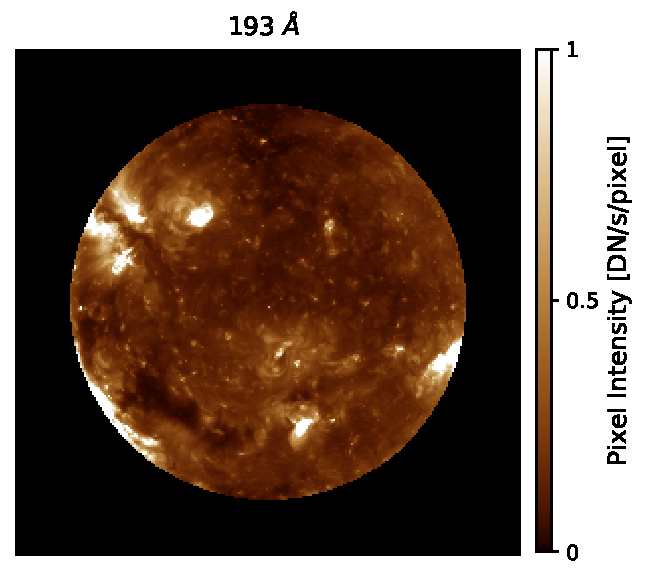
\includegraphics[width=0.8\linewidth]{reference.pdf}
  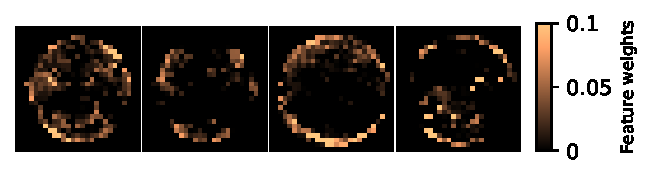
\includegraphics[width=\linewidth]{latent.pdf}
  \caption{Feature maps obtained from the last layer of CNN of our model. Top row shows a sample input in AIA 193~\AA~ channel, and the bottom row shows four representative feature maps out of one hundred and twenty eight different feature maps from the final convolutional layer of the multi-channel NN model.}
  \label{fig:autocalibrate_activation_viz}
\end{figure}


\section{Concluding remarks}
\label{section:summary}
This paper establishes the framework for a novel technique to calibrate EUV instrument degradation and advance our understanding of the cross-relation between different EUV channels. We began with formulating the problem and setting up a toy problem to test our theories. We then establish two CNNs architectures that take multiple wavelengths as input to auto-correct for on-orbit degradation of the SDO/AIA telescope. We train the model using SDOML dataset and augmented the training set by randomly degrading images at each epoch. We also shuffled images to avoid any time sequence bias. Together with the CNNs, we developed a non-machine learning baseline to benchmark and to compare with the CNNs models. Finally, we tested the CNN models on the dimming factor reconstruction error and we predicted the channels' degradation curve through time and compared it with the degradation curves V8 and V9.

The CNN approach significantly outperforms a traditional (not machine-learning based) baseline model (85\% vs. 51\% in terms of TP rate metric), for a tolerance level of 0.05. A multi-channel CNN also outperforms the single-channel CNN. This is consistent with expectations that correlations between structures in different channels, and correlations between size/morphology of structures and brightness can be used to correct degradation. A more intensive work needs to be done to understand the relationship between different channels, and which channels are related to each other. We could use the feature maps to understand how the filters are being activated through the process, and this lays down a future path for a better understanding.

The CNN models also reproduce very closely and within their error the most recent sounding-rocket based degradation curves (V8 and V9). This is particularly remarkable given no time information has been used in the training of the model. For some specific channels, like 94\AA, the model could reproduce the V8 curve well since the SDOML was corrected using this curve. We could also observe that the Single-Channel model could perform as well as the Multi-Channel model even though the multi-channel presented a more robust performance when tested before.

This work raises the possibility of auto-calibrating deep space EUV instruments (e.g., the EUV images on NASA STEREO spacecraft), which cannot be calibrated using sounding rockets (as is the case for SDO). We envision the technique presented here may also be adapted to imagers or spectrographs operating at other wavelengths (e.g., hyperspectral Earth-oriented imagers). 

\acknowledgments

{This project was conducted during the 2019 Frontier Development Lab (FDL) program, a co-operative agreement between NASA and the SETI Institute. We wish to thank IBM for providing computing power through access to the Accelerated Computing Cloud, as well as NASA, Google Cloud and Lockheed Martin for supporting this project. L.F.G.S was supported by the National Science Foundation under Grant No. AGS-1433086. M.C.M.C. and M.J. acknowledge support from NASA’s SDO/AIA (NNG04EA00C) contract to the LMSAL. S.B  acknowledges the support from the Research Council of Norway, project number 250810, and through its Centers of Excellence scheme, project number 262622. This project was also partially performed with funding from Google Cloud Platform research credits program. We thank the NASA’s Living With a Star Program, which SDO is part of, with AIA, and HMI instruments onboard.

\software{We acknowledge for CUDA processing cuDNN \citep{cudnn}, for data analysis and processing we used \citep[Sunpy][]{Sunpy2020}, Numpy \citep{numpy}, Pandas \citep{pandas}, SciPy \citep{scipy}, scikit-image \citep{scikit-image} and scikit-learn\citep{scikit-learn}. Finally all plots were done using Matplotlib \citep{matplotlib} and Astropy \citep{astropy:2018}}.}


\bibliography{autocalibration}
\bibliographystyle{aasjournal}


\newpage
\appendix
\section{Scaling Units for each AIA channel}
\label{section:appendix_average}

\begin{table}[ht]
  \centering
  \caption{Table of the scaling units of  AIA channels.}
  \label{tab:average_channels}
  \begin{tabular}{cc}
    \toprule
     AIA channel (\AA) &  Scaling unit [DN/s/pixel] \\
     \midrule
       94 &   10  \\
      131 &   80  \\
      171 & 2000  \\
      193 & 3000  \\
      211 & 1000  \\
      304 &  500  \\
      335 &   80  \\
      \bottomrule
  \end{tabular}
\end{table}


\end{document}